% Source: TeX Live tkz-fct manual, TKZdoc-fct-fonctions.tex
\documentclass[border=2pt]{standalone}
\usepackage{tkz-fct}
\begin{document}
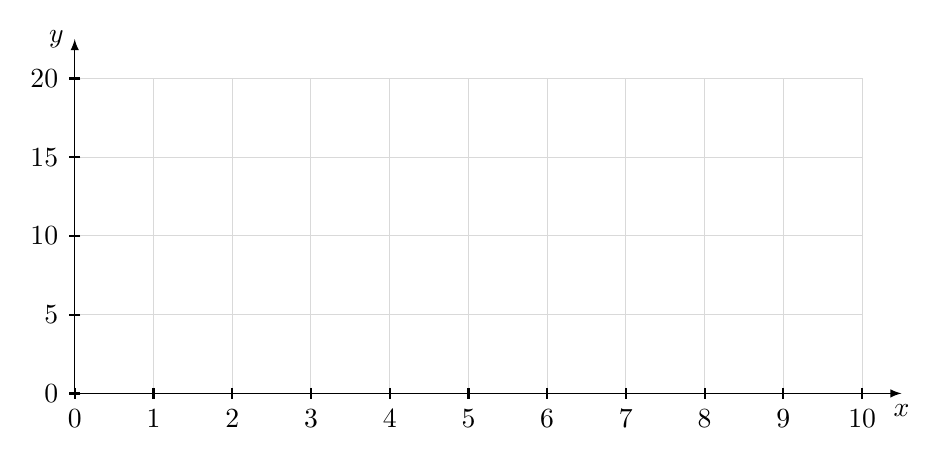
\begin{tikzpicture}
  \tkzInit[xmin=0,xmax=10,ymin=0,ymax=20,ystep=5]
  \tkzGrid[color=gray!30]
  \tkzAxeXY
  \tkzFct[color=red,domain=0:10,samples=2]{2*x+5}
  \tkzFct[color=blue,style=dashed,domain=0:10,samples=2]{-x+15}
  \tkzFct[color=green,domain=0:10,samples=2]{7}
\end{tikzpicture}
\end{document}
